
\begin{figure}[H]
  {
    \setlength{\tabcolsep}{3.0pt}
    \setlength\cmidrulewidth{\heavyrulewidth} % Make cmidrule = 
    \begin{adjustbox}{height=5cm,center}
      \footnotesize
      \begin{tabular}{ll}

        \makecell[l]{
\icode{.BYTE \$00,\$01,\$FF}\\
\icode{.BYTE \$FF,\$00,\$00}
} & \makecell[l]{

\includegraphics[width=1.3cm]{src/patterns/pixels/pixel_pattern4_0.png}%
} \\
        \midrule

        \makecell[l]{
\icode{.BYTE \$00}\\
\icode{.BYTE \$00}
} & \makecell[l]{

\includegraphics[width=1.3cm]{src/patterns/pixels/pixel_pattern4_1.png}%

\includegraphics[width=1.3cm]{src/patterns/pixels/pixel_pattern4_2.png}%
} \\
        \midrule

        \makecell[l]{
\icode{.BYTE \$00,\$01,\$02,\$FE,\$FF}\\
\icode{.BYTE \$FE,\$FF,\$00,\$00,\$FF}
} & \makecell[l]{

\includegraphics[width=1.3cm]{src/patterns/pixels/pixel_pattern4_3.png}%

\includegraphics[width=1.3cm]{src/patterns/pixels/pixel_pattern4_4.png}%

\includegraphics[width=1.3cm]{src/patterns/pixels/pixel_pattern4_5.png}%
} \\
        \midrule

        \makecell[l]{
\icode{.BYTE \$00,\$03,\$FD}\\
\icode{.BYTE \$FD,\$01,\$01}
} & \makecell[l]{
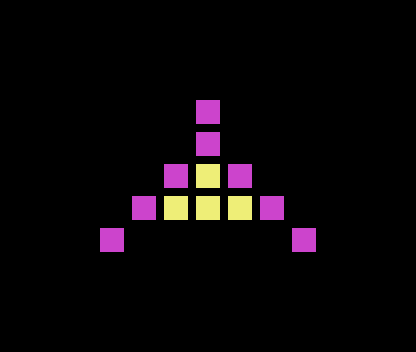
\includegraphics[width=1.3cm]{src/patterns/pixels/pixel_pattern4_6.png}%
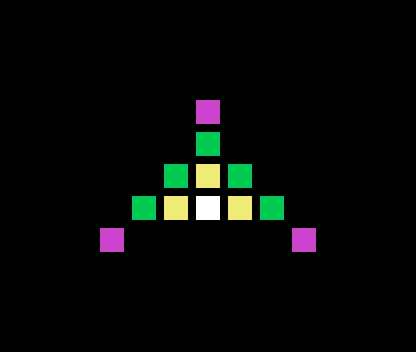
\includegraphics[width=1.3cm]{src/patterns/pixels/pixel_pattern4_7.png}%

\includegraphics[width=1.3cm]{src/patterns/pixels/pixel_pattern4_8.png}%
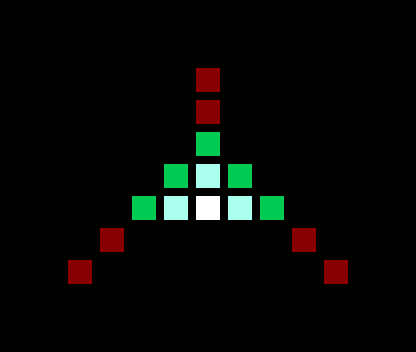
\includegraphics[width=1.3cm]{src/patterns/pixels/pixel_pattern4_9.png}%
} \\
        \midrule

        \makecell[l]{
\icode{.BYTE \$00,\$04,\$FC}\\
\icode{.BYTE \$FC,\$02,\$02}
} & \makecell[l]{
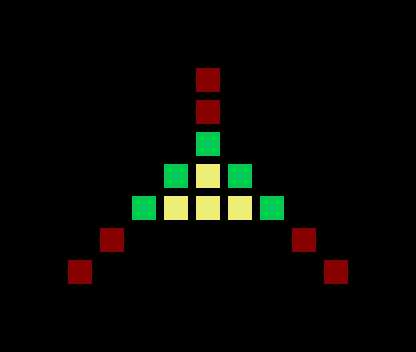
\includegraphics[width=1.3cm]{src/patterns/pixels/pixel_pattern4_10.png}%
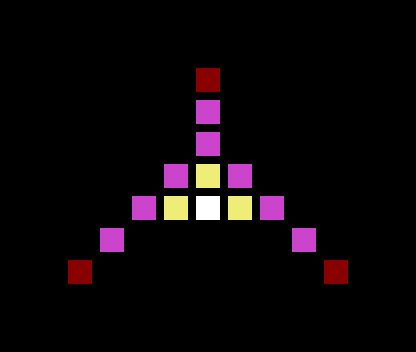
\includegraphics[width=1.3cm]{src/patterns/pixels/pixel_pattern4_11.png}%
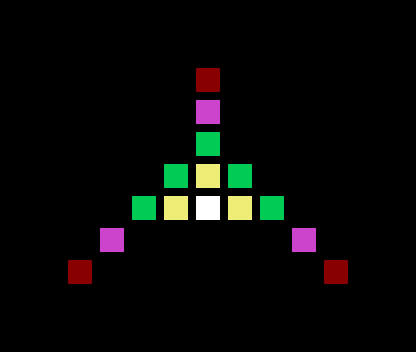
\includegraphics[width=1.3cm]{src/patterns/pixels/pixel_pattern4_12.png}%
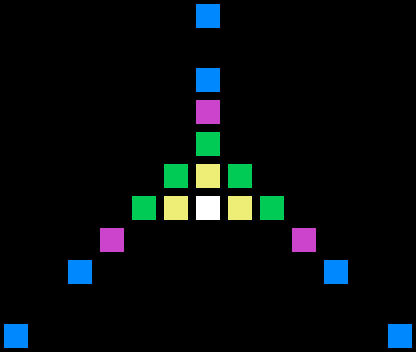
\includegraphics[width=1.3cm]{src/patterns/pixels/pixel_pattern4_13.png}%
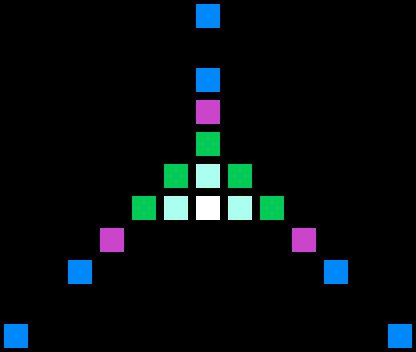
\includegraphics[width=1.3cm]{src/patterns/pixels/pixel_pattern4_14.png}%
} \\
        \midrule

        \makecell[l]{
\icode{.BYTE \$00,\$06,\$FA}\\
\icode{.BYTE \$FA,\$04,\$04}
} & \makecell[l]{
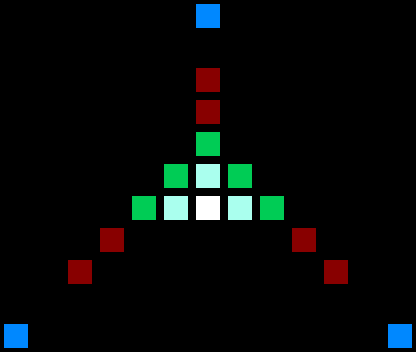
\includegraphics[width=1.3cm]{src/patterns/pixels/pixel_pattern4_15.png}%
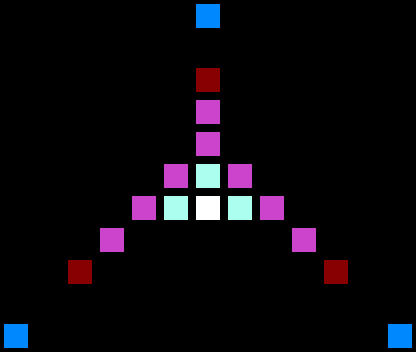
\includegraphics[width=1.3cm]{src/patterns/pixels/pixel_pattern4_16.png}%
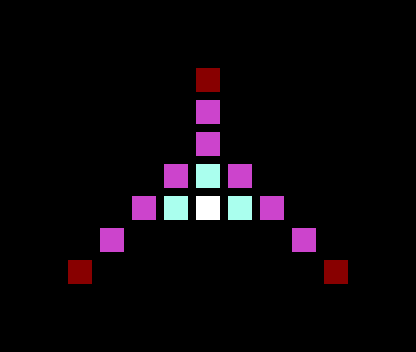
\includegraphics[width=1.3cm]{src/patterns/pixels/pixel_pattern4_17.png}%
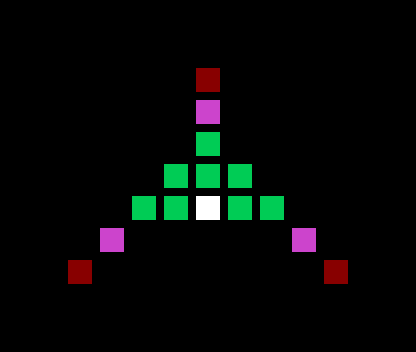
\includegraphics[width=1.3cm]{src/patterns/pixels/pixel_pattern4_18.png}%
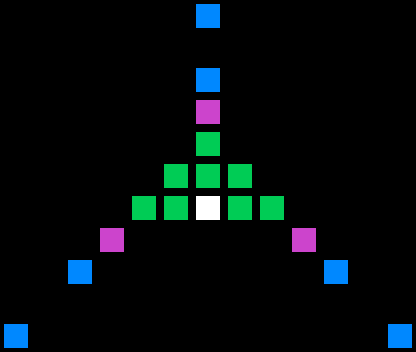
\includegraphics[width=1.3cm]{src/patterns/pixels/pixel_pattern4_19.png}%
} \\
        \midrule

        \makecell[l]{
\icode{.BYTE \$00}\\
\icode{.BYTE \$00}
} & \makecell[l]{
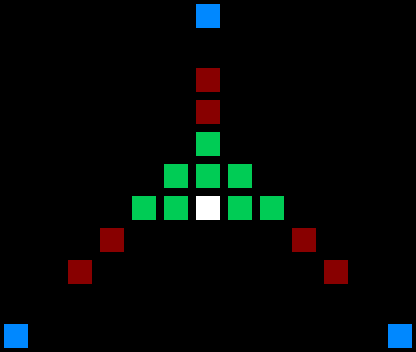
\includegraphics[width=1.3cm]{src/patterns/pixels/pixel_pattern4_20.png}%
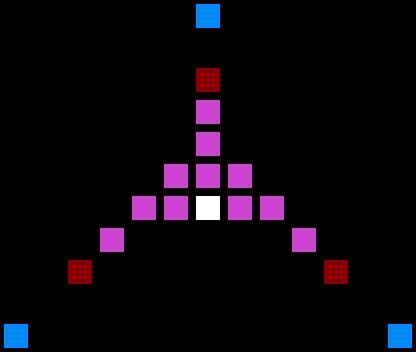
\includegraphics[width=1.3cm]{src/patterns/pixels/pixel_pattern4_21.png}%
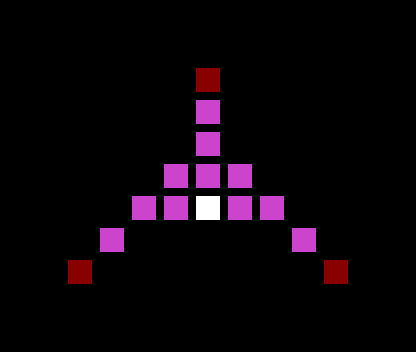
\includegraphics[width=1.3cm]{src/patterns/pixels/pixel_pattern4_22.png}%
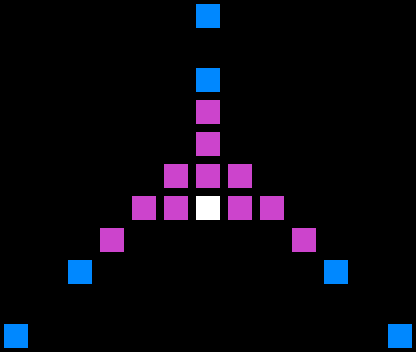
\includegraphics[width=1.3cm]{src/patterns/pixels/pixel_pattern4_23.png}%
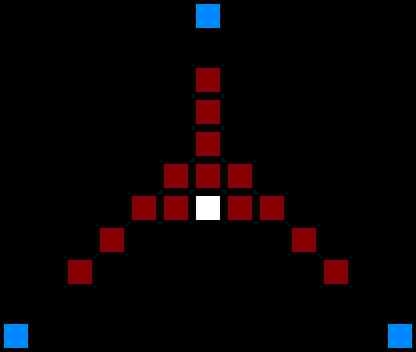
\includegraphics[width=1.3cm]{src/patterns/pixels/pixel_pattern4_24.png}%
} \\
        \midrule

      \end{tabular}
    \end{adjustbox}
  }\caption{The purpose of each of the oscillator values.}
\end{figure}
